\documentclass[conference]{IEEEtran}
\IEEEoverridecommandlockouts
% The preceding line is only needed to identify funding in the first footnote. If that is unneeded, please comment it out.
\usepackage{cite}
\usepackage{amsmath,amssymb,amsfonts}
\usepackage{algorithm}
\usepackage{algorithmic}
\usepackage{graphicx}
\graphicspath{{evals/data/metrics/figures/final/}}
\usepackage{textcomp}
\usepackage{xcolor}
\usepackage{array}
\usepackage{booktabs}
\usepackage[most]{tcolorbox}

% Churkin Protocol: Color Palette (Harmonious & Minimal)
\definecolor{churkinpurple}{RGB}{94,45,121}    % #5E2D79 (for State)
\definecolor{statusgreen}{RGB}{34,139,34}      % #228B22 (Green for True - Success)
\definecolor{statusred}{RGB}{255,99,71}       % #FF6347 (Light Red/Tomato for False - Stop/Suppressed)
\def\BibTeX{{\rm B\kern-.05em{\sc i\kern-.025em b}\kern-.08em
    T\kern-.1667em\lower.7ex\hbox{E}\kern-.125emX}}

\begin{document}

\title{EXAIM: Explainable AI Middleware for Real-Time Multi-Agent Clinical Decision Support}

\author{\IEEEauthorblockN{Abem Kibatu Woldesenbet}
\IEEEauthorblockA{\textit{The Beacom College of Computer \& Cyber Sciences} \\
\textit{Dakota State University}\\
Madison, SD, USA \\
abem.woldesenbet@trojans.dsu.edu}
\and
\IEEEauthorblockN{Andy Behrens, PhD}
\IEEEauthorblockA{\textit{Information Systems, College of Business \& Information Systems} \\
\textit{Dakota State University}\\
Madison, SD, USA \\
andy.behrens@dsu.edu}
}

\maketitle

\begin{abstract}
 Clinical decision support systems (CDSS) employing multi-agent architectures achieve high diagnostic performance but face a critical transparency bottleneck: they generate verbose, interleaved reasoning traces that are difficult for clinicians to interpret in real time. We present EXAIM (Explainable AI Middleware), an IT artifact developed under a design science research paradigm that transforms live reasoning streams into structured, concise summaries. EXAIM addresses the transparency-usability gap through three primitives: TokenGate for syntax-aware stream regulation, BufferAgent for semantic event detection, and SummarizerAgent for schema-constrained synthesis aligned with clinical frameworks (SBAR/SOAP) \cite{haig2006sbar,podder2023soap}. In contrast to post-hoc methods, EXAIM operates incrementally, triggering updates based on information novelty rather than fixed intervals. We evaluate the artifact through systematic ablation, parameter calibration, and trace-level analysis on 40 diagnostic cases, verifying that event-driven summarization improves semantic coverage relative to structural baselines while reducing redundant updates.
\end{abstract}

\begin{IEEEkeywords}
Explainable AI, Multi-agent systems, Clinical decision support, Real-time summarization, Schema-constrained summarization, Event-driven summarization
\end{IEEEkeywords}

\section{Introduction}

Multi-agent large language model (LLM) systems are increasingly explored as a clinical decision-support paradigm in which multiple role-specialized agents collaborate to reason over a case \cite{peng2025tree}, often motivated by multidisciplinary consultation workflows \cite{chenx2025diagnostic}. Prior work frames these systems as a path toward more capable diagnostic reasoning on complex cases \cite{peng2025tree}, and reports that multi-agent consultation can yield substantially larger conversational outputs than single-agent setups \cite{chenx2025diagnostic}. However, increasing output volume and interleaving across agents create a transparency tension in time-constrained settings: the information a clinician would need to inspect is dispersed across long, evolving traces rather than consolidated into stable, decision-oriented updates. This is not only an interface problem; human-grounded evidence shows that explanation complexity can impair users’ ability to simulate and apply a model’s reasoning when explanations are longer or more demanding \cite{lage2019interpretability}. Separately, CDSS adoption is sensitive to workflow fit and interruption burden, including alert fatigue \cite{sutton2020cdss} and other implementation barriers observed in qualitative syntheses \cite{derksen2025cdss}.

In a typical multi-agent session, information required for a clinical decision is dispersed across long, evolving dialogue streams rather than consolidated into stable updates. This creates a fundamental usability barrier. Clinicians operating under time pressure cannot parse raw "chain-of-thought" streams without experiencing information overload---a cognitive burden analogous to "alert fatigue" \cite{sutton2020cdss}. Furthermore, traditional post-hoc Explainable AI (XAI) methods, such as feature attribution (e.g., SHAP or LIME), are ill-suited for this domain. They typically generate explanations only after a model has completed its execution, lacking the temporal immediacy required for real-time monitoring \cite{abbas2025xai}.

To address these challenges, we develop EXAIM (Explainable AI Middleware), an IT artifact constructed under a design science research (DSR) paradigm that transforms opaque multi-agent text streams into transparent, clinically actionable summaries.

EXAIM achieves this transformation through three architectural innovations: (1) syntax-aware stream regulation (TokenGate), which segments bursty token streams into coherent linguistic units to prevent fragmentation; (2) semantic event detection (BufferAgent), which filters updates based on completeness, relevance, and novelty to reduce redundant interruptions; and (3) schema-constrained synthesis (SummarizerAgent), which enforces strict output contracts aligned with SBAR/SOAP communication standards to guarantee consistent interface utility.


The following research question guides the evaluation of this artifact:

	\textbf{RQ1:} Can event-driven, schema-constrained summarization improve trace utility by increasing semantic coverage while reducing redundant updates?

We operationalize RQ1 through four sub-questions corresponding to distinct evaluation dimensions:
\begin{itemize}
\item \textbf{RQ1a:} Does EXAIM improve trace coverage under identical schema and peer-summary character constraints compared to structural triggers?
\item \textbf{RQ1b:} Does EXAIM reduce redundant and low-novelty updates through semantic buffering and novelty filtering?
\item \textbf{RQ1c:} Does EXAIM preserve contract-grounded faithfulness when limited continuity across summaries is permitted?
\item \textbf{RQ1d:} What impact does semantic event detection introduce relative to simpler triggers such as turn boundaries or fixed-interval chunking?
\end{itemize}

To evaluate these questions, we conducted an ablation study in which we instantiated a real-time summarization middleware that intercepts LLM reasoning traces and emits structured summaries constrained by a fixed schema. The artifact enables controlled variation of triggering strategies (event-driven versus baseline triggers), continuity constraints, and update policies, allowing systematic assessment of their effects on semantic coverage, redundancy, faithfulness, and computational overhead.

This paper makes the following contributions:
\begin{itemize}
\item \textbf{We develop a modular middleware architecture} that transforms streaming multi-agent reasoning traces into structured, clinician-aligned summaries, optimizing information density and reducing alert frequency in real-time CDSS.
\item \textbf{We introduce a semantic buffering mechanism} that detects topic shifts, novelty, and critical clinical events to trigger summaries based on context, thereby reducing irrelevant interruptions relative to turn-based baselines.
\item \textbf{We demonstrate process-level transparency} through structured summaries aligned with SBAR/SOAP communication patterns, designed to preserve agent attribution and uncertainty while enforcing strict brevity constraints.
\item \textbf{We formalize the impact of semantic buffering} on coverage, redundancy, faithfulness, and computational cost through a systematic ablation study on 40 diagnostic cases.
\end{itemize}

The remainder of this paper is organized as follows. Section II positions EXAIM within the XAI-CDSS and streaming summarization literature and synthesizes design gaps. Section III details the DSR-guided artifact, its three modules, and provides a demonstrative case walkthrough. Section~\ref{sec:experiments} describes the trace replay dataset, calibration procedure, and ablation experiments, reporting quantitative results. Section V interprets findings via design implications and deployment considerations. Section VI concludes and outlines future work.


\section{Literature Review}

\subsection{Multi-Agent LLM CDSS and the Trace Consumption Problem}
Recent multi-agent approaches frame clinical reasoning as collaboration among specialized roles \cite{peng2025tree}, including consultation metaphors inspired by multidisciplinary teams \cite{chenx2025diagnostic}. A practical implication of these designs is increased output volume: a multi-agent consultation framework can “allow for significantly more output tokens” than single-agent settings \cite{chenx2025diagnostic}. Separately, explainable multi-agent clinical reasoning systems emphasize that black-box medical decision-making can undermine trust and impede effective care processes \cite{hong2024argmed}. What this literature establishes is that multi-agent reasoning is a plausible technical route to richer clinical deliberation, and that explainability is central for acceptance in clinical decision workflows. What it does not resolve is how to mediate long, interleaved, evolving traces into stable, time-efficient updates for downstream consumption. EXAIM is positioned specifically at this interface: it treats the trace as a streaming artifact that must be shaped for human attention and workflow constraints.

\subsection{Explainability in CDSS: Methods Are Common; Delivery Constraints Remain Under-Specified}
A broad CDSS XAI meta-analysis catalogs commonly used interpretability methods in the CDSS literature, including feature-attribution families such as SHAP and LIME among other technique classes \cite{abbas2025xai}. The same synthesis emphasizes that explanation effectiveness depends not only on method choice but on user-centered delivery factors: explanation timing influences trust, and granularity can affect trust and cognitive load \cite{abbas2025xai}. In practice, CDSS deployment is repeatedly constrained by workflow integration issues and interruption burdens, including alert fatigue \cite{sutton2020cdss}. Human-subject evidence outside clinical settings further motivates bounded explanations: increasing explanation complexity can degrade users’ ability to simulate and apply a model’s logic \cite{lage2019interpretability}. EXAIM translates these constraints into system requirements: explanations must be (i) delivered incrementally at meaningful points, (ii) brief enough to be usable under time pressure, and (iii) stable enough to avoid unnecessary cognitive churn.

\subsection{Online and Real-Time Summarization: Update Policies, Rewrite Costs, and Stability}
Online summarization differs from offline summarization in fundamental ways \cite{schneider2024meeting}, because the system must decide both when to write and how to revise what has been written. Importantly, revision is not “free”: rewriting or deleting already-presented information can be cognitively straining for readers \cite{schneider2024meeting}. In real-time medical conversation summarization, Le-Duc et al. produce local summaries at fixed intervals (``after each N utterances'') \cite{leduc2025speech} and explicitly note that continuously updated summaries can confuse readers because content changes constantly \cite{leduc2025speech}. These findings directly motivate EXAIM’s design choice to (a) avoid constant micro-updates, (b) detect semantically meaningful boundaries rather than relying only on fixed windows, and (c) emit updates that minimize destabilizing rewrites.

\subsection{Structured Clinical Documentation as an Output Contract}
A major adjacent line of work targets structured medical documentation from conversations. Krishna et al. explicitly aim to generate full SOAP notes with many subsections from clinical conversations paired with SOAP notes authored under documentation standards \cite{krishna2021soap}. This reinforces the utility of SOAP-style structure as an organizing schema for clinician-facing summaries. More recent annotation frameworks move beyond static transcript-summary pairs. Zhang et al. observe that the conventional transcript-summary pair format yields end-to-end models that are ``effectively blackboxes with limited interpretability'' and propose Incremental Note Generation, where annotators incrementally draft notes and later rewrite them, producing editing histories \cite{zhang2024annotate}. This supports EXAIM’s focus on incremental updates and motivates explicit notions of ``draft state'' and ``revision policy'' in the downstream interface.

Finally, usability principles for safety-critical alerting emphasize the value of constrained presentation: alerts should be "concise, understandable, and consistently structured" \cite{marcilly2018alerts}. EXAIM operationalizes this as hard schema validation plus strict budget constraints at the middleware output.

\subsection{Implications for EXAIM Design Choices}
Synthesizing the above, the literature motivates three design commitments that are not jointly addressed by prior work: (1) stream mediation for long, interleaved multi-agent traces \cite{chenx2025diagnostic}, (2) delivery-aware explainability that accounts for timing and granularity constraints \cite{abbas2025xai} and workflow interruption costs \cite{sutton2020cdss}, and (3) stability under revision, given evidence that rewriting can be cognitively costly and continuous updates can confuse readers \cite{schneider2024meeting,leduc2025speech}. EXAIM’s TokenGate, BufferAgent, and SummarizerAgent are organized to satisfy these constraints by regulating inputs, triggering updates on semantically meaningful events, and enforcing schema/budgeted outputs aligned with SOAP-style consumption \cite{krishna2021soap}.
To ensure the utility of summaries, they must conform to established mental models. Krishna et al. \cite{krishna2021soap} demonstrate the efficacy of generating SOAP notes (Subjective, Objective, Assessment, Plan) from clinical conversations, reinforcing the utility of this structure for clinician-facing summaries. However, standard transcript-summary pairs often yield "black box" end-to-end models \cite{zhang2024annotate}. By contrast, incremental generation frameworks suggest that notes should evolve. Usability principles for safety-critical alerting further emphasize that alerts must be "concise, understandable, and consistently structured" \cite{marcilly2018alerts}. EXAIM operationalizes these insights by enforcing a strict output contract: every summary must validate against a fixed SBAR/SOAP schema, guaranteeing that the interface remains stable regardless of upstream model volatility.

\section{Artifact Description}

Design Science aims to create and evaluate IT artifacts intended to solve identified organizational problems \cite{hevner2004design}. Consistent with the principles of DSR, we develop EXAIM as a solution-oriented IT artifact designed to optimize information density and reduce alert frequency in multi-agent CDSS. This approach aligns with recent applications of DSR for developing AI-based clinical tools that balance technical innovation with practical usability requirements \cite{hor2025design}. Following the process model outlined by Peffers et al. \cite{peffers2007dsr}, this section provides a systematic description of the artifact's architecture, key components, and operational logic. We first present the overall framework, then detail the three primary modules (TokenGate, BufferAgent, SummarizerAgent), and finally demonstrate the system's operation through a case walkthrough.

\subsection{Overall Framework}
\label{sec:overall-framework}

EXAIM functions as a transparency middleware that sits between upstream diagnostic multi-agent systems and downstream clinician-facing interfaces. The core architectural challenge is straightforward: multi-agent systems generate thousands of token-level deltas per diagnostic session, yet clinicians require at most a dozen discrete, structured updates. EXAIM bridges this gap by transforming high-velocity, interleaved token streams into semantically bounded summary events.

As illustrated in Figure~\ref{fig:system-architecture}, the system accepts an asynchronous stream of token deltas $D = \{(a_t, \tau_t)\}_{t=1}^T$, where each delta consists of an agent identifier $a_t$ and a text fragment $\tau_t$. This input model is deliberately agnostic to the underlying agent architecture---EXAIM requires only that agents emit text incrementally, making it compatible with any streaming LLM framework.

The system emits a sequence of structured summary objects $S = \{s_1, s_2, \ldots, s_N\}$, where each $s_i$ conforms to a strict JSON schema mapped to clinical communication standards (SBAR/SOAP). Critically, $N \ll T$, representing a meaningful reduction in event frequency.

Four explicit design objectives constrain the system's behavior and provide the criteria against which ablation variants are evaluated. The primary concern is managing update frequency: the system prioritizes fewer, higher-information summaries per case, treating update count as a constrained resource rather than maximizing raw coverage at the cost of interruption burden. Complementing this, strict schema compliance with bounded character budgets guarantees a stable UI footprint, ensuring that all outputs validate against the AgentSummary schema or are discarded. To preserve the integrity of the upstream diagnostic process, middleware processing occurs asynchronously in a ``sidecar'' pattern, and EXAIM is architected to avoid adding latency to agent generation. Finally, summaries must be generated solely from buffered trace content and limited history ($k=3$ prior summaries), explicitly prohibiting external knowledge retrieval. Together, these constraints reflect a fundamental design philosophy: EXAIM does not attempt to ``improve'' the diagnostic reasoning but rather to make it transparently observable.

\begin{figure*}[htbp]
    \centering
    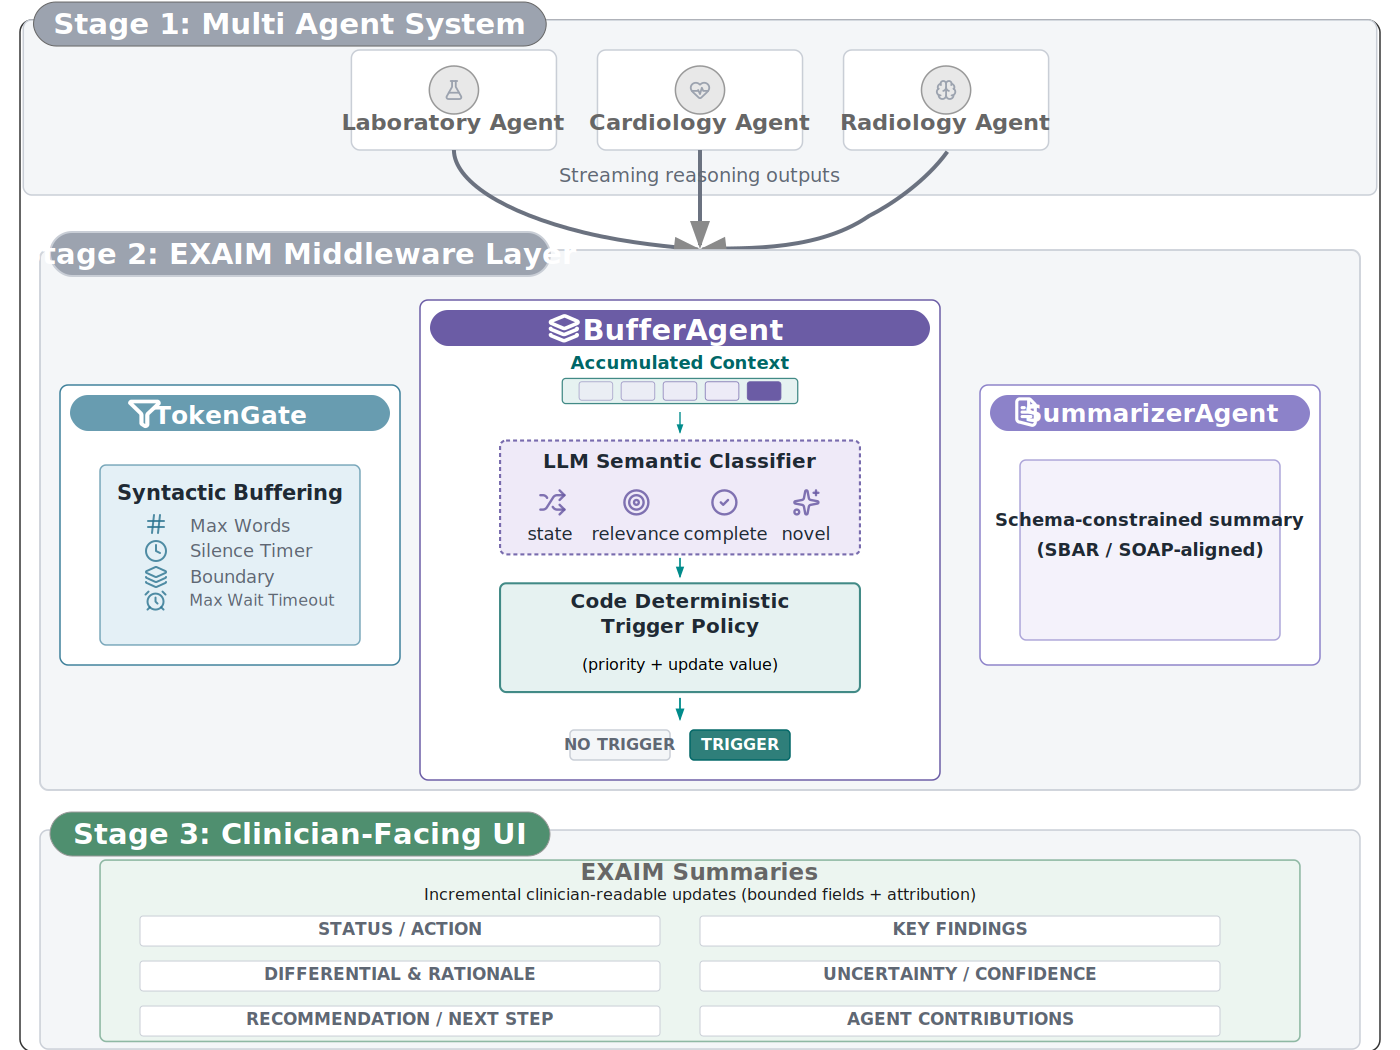
\includegraphics[width=\textwidth]{../raw/systemFigure/system.pdf}
    \caption{EXAIM middleware: converts interleaved multi-agent reasoning into concise, schema-aligned SBAR/SOAP summaries.}
    \label{fig:system-architecture}
\end{figure*}


\subsection{TokenGate: Syntax-Aware Stream Regulation}

Raw LLM token streams arrive in unpredictable bursts. In a typical multi-agent diagnostic session, a single agent might emit individual characters during deliberation, then suddenly flush complete paragraphs when reaching a conclusion. This fragmentation creates a fundamental challenge for semantic analysis: to detect topic shifts or assess novelty, the system requires coherent linguistic units---complete clauses or sentences---but the raw stream provides no such boundaries.

TokenGate implements a stateful accumulation buffer that flushes under one of four compactly specified conditions to balance linguistic coherence and responsiveness: (1) a boundary-aware flush when the buffer has at least $w_{\text{min}}$ words and ends with terminal punctuation; (2) a hard-limit flush when the buffer exceeds $w_{\text{max}}$ words regardless of punctuation; (3) a silence timeout flush if the agent is silent for more than $t_{\text{silence}}$ seconds while the buffer contains at least $w_{\text{min}}$ words; and (4) a safety-valve flush if total wait time surpasses $t_{\text{max}}$ since the first delta. These parameters ($w_{\text{min}}$, $w_{\text{max}}$, $t_{\text{silence}}$, $t_{\text{max}}$) jointly determine the Pareto frontier between linguistic coherence and real-time responsiveness. Section~\ref{sec:calibration} describes the systematic calibration procedure used to identify optimal values.

\subsection{BufferAgent: Semantic Event Detection}

If TokenGate solves the syntactic segmentation problem, BufferAgent solves the semantic filtering problem. Not every coherent chunk of agent reasoning deserves to interrupt the clinician. An agent might spend several sentences re-stating background knowledge, concurring with a previous diagnosis, or exploring a hypothesis already ruled out by others. Presenting all such content as discrete updates would recreate the very cognitive overload EXAIM aims to prevent.

BufferAgent acts as the system's cognitive filter, analyzing each chunk from TokenGate to determine whether it merits triggering a summary. The decision process operates in two stages, deliberately separating semantic interpretation (performed by an LLM) from control logic (executed by deterministic code). This separation ensures that while the system leverages language model capabilities for content understanding, the final trigger decision remains auditable and explainable.

When a chunk $C$ arrives, BufferAgent invokes an LLM classifier to extract four semantic predicates: \textbf{Complete}, \textbf{Relevant}, \textbf{Novel}, and \textbf{State} (continuation, topic shift, or critical alert). These feed a deterministic trigger decision:
\[
T = \begin{cases}
\text{True} & \text{if } \mathit{State} = \text{CRITICAL} \\
\text{True} & \text{if } \mathit{Complete} \land \mathit{Relevant} \land \mathit{Novel} \\
\text{True} & \text{if } (\mathit{State} = \text{SHIFT}) \land \mathit{Relevant} \land \mathit{Novel} \\
\text{False} & \text{otherwise}
\end{cases}
\]
This encodes a hypothesis that clinicians need immediate critical alerts, comprehensive novel conclusions, and topic transitions---but not incremental deliberation or redundant restatements.

\subsection{SummarizerAgent: Schema-Constrained Synthesis}

When BufferAgent determines that a chunk merits clinician attention, SummarizerAgent faces the final transformation challenge: compressing potentially verbose agent reasoning into a rigid, scannable format aligned with clinical communication standards. This component embodies the system's commitment to interface stability---no matter how chaotic or verbose the upstream reasoning, the output must conform to a bounded schema that downstream UIs can reliably render.

The agent receives three inputs: the triggering chunk $C$, the agent context (identifier and role), and a sliding window of the three most recent summaries $H_{k=3}$. This limited history serves dual purposes---it enables the summarizer to avoid repeating recently stated information while providing continuity for multi-turn reasoning threads.

Generation employs a three-attempt validation strategy to guarantee schema compliance. The LLM first generates structured output using strict Pydantic type definitions with schema enforcement (strict=True) mapped to SBAR/SOAP fields (Table~\ref{tab:schema}). If character limits are exceeded, the system creates a targeted rewrite prompt identifying the violating fields and their required length reductions, then re-invokes the LLM. Should validation still fail after this rewrite attempt, the system applies hard truncation at character boundaries as a final fallback.

This schema-first approach differs fundamentally from unconstrained summarization, which optimizes for semantic coverage or fluency but provides no length guarantees. EXAIM inverts this priority: the AgentSummary schema (Table~\ref{tab:schema}) enforces a structured contract between the middleware and clinician-facing interfaces, mapping each field to SBAR/SOAP clinical communication frameworks. Character budgets are non-negotiable constraints derived from UI layout requirements---brief field lengths force scannability, field semantics mirror clinical documentation workflows, and hard limits guarantee stable UI footprint regardless of model verbosity.

\begin{table*}[htbp]
\caption{EXAIM Summary Schema: Clinical Mapping and Bounded Output Budgets}
\label{tab:schema}
\begin{center}
\renewcommand{\arraystretch}{1.3}
\begin{tabular}{p{2.5cm}p{2.5cm}p{4cm}p{1.5cm}p{4.5cm}}
\toprule
\textbf{Field} & \textbf{Clinical Map} & \textbf{Role} & \textbf{Budget (Chars)} & \textbf{Design Motivation} \\
\midrule
Status / Action & SBAR: Situation & Alert header; scannable update. & 150 chars & Enforces scannability via brief title heuristic \cite{pourian2025alerts}. \\
Key Findings & SOAP: Obj/Subj & Salient facts; ``live snippet'' paradigm. & 180 chars & Supports $\sim$2 concise snippets aligned with targeted summarization limits \cite{vanveen2023summarization}. Structured presentation addresses transparency barriers identified in patient-centered CDSS deployment \cite{harrison2022patient}. \\
Differential & SOAP: Assessment & Diagnostic interpretation. & 210 chars & Bounds complexity to maintain interpretability \cite{lage2019interpretability}. \\
Uncertainty & SOAP: Assessment & Explicit confidence signal. & 120 chars & Simplified framing for trust calibration \cite{goel2022covid}. \\
Rec. / Plan & SOAP: Plan & Actionable next step. & 180 chars & Action-linked explanations \cite{silva2023xai}. \\
Agent Contrib. & System Meta & Attribution of active agents. & 150 chars & Pipeline transparency patterns \cite{donadello2021sexai}. \\
\bottomrule
\end{tabular}
\end{center}
\end{table*}

\subsection{Demonstrative Case Walkthrough}

We illustrate EXAIM's redundancy detection using Case ID 3949 from the MAC Framework (Section~\ref{sec:data}). At this point in the trace, doctor0 and doctor1 had established Spinocerebellar Ataxia (SCA) as the leading diagnosis, and the middleware had already captured this consensus. When doctor2 entered with a verbose response---``\textit{I concur with both Doctor0 and Doctor1. The gradual onset at age 30 years aligns with hereditary SCA...}''---the dashboard remained static (Fig.~\ref{fig:suppression-demo}) while BufferAgent's multi-stage evaluation (Fig.~\ref{fig:logic-card}) detected semantic redundancy: despite clinical relevance, the novelty check failed, suppressing the update. Only when doctor2 introduced genuinely new details (``High-Resolution MRI techniques,'' ``Oligoclonal bands'') did the system trigger a consolidated summary.

\begin{figure}[h]
    \centering
    \scalebox{0.65}{%
    \begin{tcolorbox}[
        enhanced,
        colback=white,
        colframe=black,
        boxrule=0.5mm,
        arc=2mm,
        drop shadow,
        left=4mm,
        right=4mm,
        top=2mm,
        bottom=2mm,
        title=\textbf{BufferAgent Status [doctor2]},
        fonttitle=\bfseries\normalsize,
        coltitle=black,
        colbacktitle=white,
        halign title=center,
        fontupper=\normalsize
    ]
        \normalsize
        
        \textbf{Input Stream:}
        \vspace{-1mm}
        \begin{quote}
            \itshape "...I concur with both Doctor0 and Doctor1... adding no new information."
        \end{quote}
        \vspace{1.5mm}
        
        \textbf{Decision Flags:}
        \vspace{0.5mm}
        
        \begin{center}
        \begin{tabular}{@{}c@{}}
            \raisebox{5pt}{State} \\
            \tcbox[colback=churkinpurple!15, colframe=churkinpurple, size=small, boxrule=0.5mm, left=2mm, right=2mm, top=0.5mm, bottom=0.5mm, fontupper=\normalsize]{\textcolor{churkinpurple}{\texttt{SAME\_TOPIC\_CONTINUING}}}
        \end{tabular}
        \end{center}
        
        \vspace{0.1mm}
        \begin{center}
        \begin{tabular}{@{}c@{\hspace{2mm}}c@{\hspace{2mm}}c@{}}
            \begin{tabular}{@{}c@{}}
                \raisebox{5pt}{Complete} \\[-3pt]
                \tcbox[colback=statusgreen!15, colframe=statusgreen, size=small, boxrule=0.5mm, left=2mm, right=2mm, top=0.2mm, bottom=0.2mm, fontupper=\normalsize]{\textcolor{statusgreen}{\textbf{True}}}
            \end{tabular} &
            \begin{tabular}{@{}c@{}}
                \raisebox{5pt}{Relevant} \\[-3pt]
                \tcbox[colback=statusgreen!15, colframe=statusgreen, size=small, boxrule=0.5mm, left=2mm, right=2mm, top=0.2mm, bottom=0.2mm, fontupper=\normalsize]{\textcolor{statusgreen}{\textbf{True}}}
            \end{tabular} &
            \begin{tabular}{@{}c@{}}
                \raisebox{5pt}{Novel} \\[-3pt]
                \tcbox[colback=statusred!15, colframe=statusred, size=small, boxrule=0.5mm, left=2mm, right=2mm, top=0.2mm, bottom=0.2mm, fontupper=\normalsize]{\textcolor{statusred}{\textbf{False}}}
            \end{tabular} \\
        \end{tabular}
        \end{center}
        \vspace{-2mm}
        \begin{center}
            $\downarrow$
        \end{center}
        \vspace{-2mm}
        \begin{center}
            \tcbox[
                enhanced,
                colback=statusred!20,
                colframe=statusred,
                boxrule=0.5mm,
                size=normal,
                fontupper=\bfseries\normalsize,
                left=3mm,
                right=3mm,
                top=0.5mm,
                bottom=0.5mm
            ]{\textcolor{statusred}{Trigger = False (Suppressed)}}
        \end{center}
        
        \vspace{0.1mm}
        \noindent\rule{\linewidth}{0.5mm}
        \vspace{0.5mm}
        
        \textbf{Rationale:} Doctor2 concurs with SCA based on ataxia/dysarthria/MRI... adding no new information. The content is \textcolor{statusgreen}{relevant} as it details planned actions, but it is \textcolor{statusred}{not novel} as these details were already broadly mentioned in previous summaries.
    \end{tcolorbox}%
    }
    \caption{BufferAgent System Status Card showing the hierarchical decision logic.}
    \label{fig:logic-card}
\end{figure}

\begin{figure*}[htbp]
\centering
\scalebox{1}{%
\includegraphics[width=\textwidth]{case_walkthrough/CaseWalkthroughImage.png}%
}
\caption{EXAIM dashboard during redundancy suppression: the incoming raw stream (left) is suppressed, leaving the displayed summary (right) unchanged.}
\label{fig:suppression-demo}
\end{figure*}

\section{Experiments and Results}
\label{sec:experiments}

We verify the effectiveness of the EXAIM artifact through a "glass-box" evaluation methodology using deterministic replays of multi-agent reasoning traces. This approach allows us to stress-test the middleware's flow-control capabilities independent of variations in upstream agent behavior.

\subsection{Data / Trace Replay Setup}
\label{sec:data}

We utilized the Multi-Agent Conversation (MAC) framework \cite{chenx2025diagnostic} as the upstream trace generator. MAC is a multi-agent diagnostic system where diverse doctor agents and a supervisor collaborate to solve complex medical cases. We executed MAC with GPT-4o-mini using the authors' default configuration without modification.

To capture realistic streaming dynamics, we instrumented MAC via a transparent OpenAI API monkeypatch that logs per-delta emissions and microsecond timestamps without altering MAC's conversation logic, speaker selection, or termination behavior. These logs serve as a frozen replay dataset of 40 rare-disease diagnostic cases from MAC's dataset (seed=42), enabling deterministic simulation of live streams.

EXAIM uses Google Gemini (gemini-2.5-flash-lite) for both BufferAgent semantic classification and SummarizerAgent schema-constrained generation. Middleware inference was executed deterministically (temperature=0.0), with other parameters left at defaults. Prompts and decoding parameters are fixed and version-pinned in the repository.

UMLS concepts (CUIs) used for metric computation were extracted with scispaCy (model = en\_core\_sci\_sm) linked to UMLS Release 2023AB; extraction applied a candidate-score threshold ($\geq 0.7$), top-K selection (K=10), and stoplist filtering for entities and CUIs.

\subsection{Ablation and Baselines}
\label{sec:ablation}

We isolate the contribution of each architectural primitive through a controlled ablation study. V1 establishes a turn-boundary baseline, summarizing only when agents complete their generations---a natural structural trigger reflecting conventional dialogue system paradigms. V2 disables BufferAgent filtering entirely, passing all TokenGate flushes directly to summarization to isolate the impact of semantic gating on update frequency and redundancy. V3 replaces TokenGate's syntax-aware segmentation with calibrated fixed-interval chunking, testing whether adaptive linguistic boundaries improve faithfulness over uniform partitioning. V4 disables only the novelty filter while preserving BufferAgent's completeness and relevance checks, isolating whether contextual redundancy detection is necessary for managing alert burden. Table~\ref{tab:ablation-variants} defines the five experimental configurations (V0--V4).

\begin{table}[htbp]
\caption{Ablation Variant Configurations}
\label{tab:ablation-variants}
\begin{center}
\renewcommand{\arraystretch}{1.3}
\begin{tabular}{lcccc}
\toprule
\textbf{Variant} & \textbf{TokenGate} & \textbf{BufferAgent} & \textbf{Novelty} \\
\midrule
V0 (Full EXAIM) & \checkmark & \checkmark & \checkmark\\
V1 (Turn-End) & $\times$ & $\times$ & N/A \\
V2 (No BufferAgent) & \checkmark & $\times$ & N/A \\
V3 (Fixed-Chunk) & $\times$ & \checkmark & \checkmark \\
& (fixed CTU) & & & \\
V4 (No Novelty) & \checkmark & \checkmark & $\times$ \\
\bottomrule
\end{tabular}
\end{center}
\footnotesize
Note: All variants use identical SummarizerAgent schema and history\_k=3 for fair comparison.
\normalsize
\end{table}

\subsection{Calibration Protocol}
\label{sec:calibration}

To ensure fair evaluation, we executed a rigorous parameter selection process before final testing:
\begin{enumerate}
    \item \textbf{TokenGate Calibration}: We performed a grid search over 625 policy combinations (varying word counts and timeouts) on the replay dataset. The final policy (min\_words=60, max\_word=100, silence=1.0s, safe\_wait=4.0s) was selected via Pareto frontier analysis to jointly optimize latency and linguistic coherence.
    \item \textbf{V3 Fixed-Chunk Calibration}: V3 chunk size was derived from V0 TokenGate regular flushes (excluding end-of-trace and turn-end) using a two-stage median: per-case median CTU, then median across the first 40 cases. This ensures V3 operates at comparable segmentation granularity to V0 while isolating the contribution of adaptive boundaries.
    \item \textbf{Measurement Standardization}: We report all token volumes and costs in \textbf{Character-Normalized Token Units (CTU)}, defined as $\lceil \text{len(text)} / 4 \rceil$, to ensure vendor-agnostic reproducibility.
\end{enumerate}
% (TokenGate parameter grid removed per request.)

% TokenGate Parameter Calibration Grid removed.

\subsection{Metrics}

We prioritized five metrics that directly quantify utility and reliability proxies:

\begin{itemize}
    \item \textbf{Window-Groundedness (M6a):} A window-grounded variant of faithfulness that measures the fraction of summary concepts grounded within a local sliding window of trace content centered on the summary's trigger:
    \begin{equation}
    M6a = \frac{1}{N}\sum_{i=1}^{N} \frac{|\text{summary\_CUIs}_i \cap \text{trace\_CUIs}_{\text{window}(i)}|}{|\text{summary\_CUIs}_i|}
    \end{equation}
    where $N$ is the number of evaluated summaries, $\text{summary\_CUIs}_i$ is the set of CUIs extracted from summary $i$, and $\text{trace\_CUIs}_{\text{window}(i)}$ denotes the set of CUIs extracted from the sliding window of trace content surrounding the trigger that produced summary $i$. M6a reflects local grounding and is less sensitive to distant context than M6b.

    \item \textbf{Strict Faithfulness (M6b):} The fraction of summary concepts grounded in the full trace:
    \begin{equation}
    M6b = \frac{|\text{summary\_CUIs} \cap \text{trace\_CUIs}|}{|\text{summary\_CUIs}|}
    \end{equation}
    Higher scores indicate stronger concept-level grounding. This metric penalizes unsupported insertions but does not account for semantic paraphrase (see Section~\ref{sec:faithfulness_limitations}). Faithfulness is a standard evaluation criterion in human-in-the-loop dialogue systems \cite{chen2022hitl}.
    \item \textbf{Redundancy Reduction (M3):} Measured via mean Jaccard similarity between consecutive summary updates:
    \begin{equation}
    M3 = \frac{1}{n-1}\sum_{i=1}^{n-1} \frac{|C_i \cap C_{i+1}|}{|C_i \cup C_{i+1}|}
    \end{equation}
    where $C_i$ and $C_{i+1}$ are the sets of unique UMLS concepts (CUIs) extracted from summaries $S_i$ and $S_{i+1}$, and $n$ is the total number of summaries. Lower scores indicate successful suppression of repetitive content.
    \item \textbf{Trace Coverage (M4):} The fraction of unique trace CUIs captured across all summaries:
    \begin{equation}
    M4 = \frac{|\bigcup_{i=1}^{n} \text{summary\_CUIs}_i \cap \text{trace\_CUIs}|}{|\text{trace\_CUIs}|}
    \end{equation}
    This metric is \emph{not normalized by update count}, and therefore inherently favors high-frequency systems. M7 (Budget Efficiency) provides the normalized coverage view.
    \item \textbf{System Latency (M8):} The end-to-end processing time (buffer analysis + summarization generation) to validate the ``real-time'' architectural claim.
    \item \textbf{Schema Compliance (M10):} The rate of successful adherence to the JSON clinical output schema, verifying the system's structural reliability.
\end{itemize}
Supplementary metrics (Update Count, Token Volume, LLM Cost) provide context for trade-off analysis.

\subsubsection{Interpretation of Concept-Level Metrics}
\label{sec:faithfulness_limitations}

Our faithfulness metrics (M6a, M6b) operate at the level of explicit concept realization rather than semantic equivalence or entailment. This introduces a fundamental mismatch: overlap-based metrics like ROUGE fail to correlate with clinical quality when models use paraphrasing rather than literal repetition \cite{fraile2025llm,bailly2025divide}.

Schema-constrained summarization necessarily introduces transformations that reduce recall under strict NER-based concept matching: abbreviation of clinical phrases (e.g., ``acute renal failure'' $\rightarrow$ ``AKI''), normalization of hedged statements and compression omitting modifiers to meet character limits \cite{yim2023acibench}, and schema remapping reorganizing facts into SBAR/SOAP slots through incremental UPDATE and REMOVE operations \cite{zhang2024annotate}.

UMLS-based NER assumes explicit lexical realization and near-literal mention of entities \cite{vanveen2023summarization,yim2023acibench}, misaligning with summaries that preserve semantic content through paraphrase. String-matching approaches demonstrate low correlation with physician preferences when content is normalized or compressed \cite{yim2023acibench,vanveen2023summarization}, causing schema-constrained summarizers to under-score even when accurately representing clinical content \cite{fraile2025llm}.

Despite these limitations, concept-level metrics remain informative for relative comparisons across ablation variants under identical extraction assumptions. Future work should incorporate clinician-judged factual consistency \cite{fraile2025llm}, entailment verification, and task-based evaluation to complement automated assessment.

\subsection{Results}


Table~\ref{tab:metrics} reports metrics related to schema compliance, faithfulness, and latency---core indicators of EXAIM's reliability as a clinician-facing interface component. We report bootstrap 95\% confidence intervals (10,000 samples, seed=42) for M4, M6a, and M6b where available.

\begin{table*}[t]
\centering
\caption{Contract and Quality Metrics (Mean [95\% CI])}
\label{tab:metrics}
\renewcommand{\arraystretch}{1.25} % Adds vertical space between rows
\setlength{\tabcolsep}{6pt}        % Adds horizontal space between columns

\begin{tabular}{l c c c c c}
\toprule  % Professional top line
\textbf{Metric} & \textbf{V0} & \textbf{V1} & \textbf{V2} & \textbf{V3} & \textbf{V4} \\
\midrule  % Professional middle line

Faithfulness \textit{(M6b)} & 0.421 & 0.333 & 0.409 & 0.382 & 0.424 \\
& [0.389, 0.453] & [0.309, 0.356] & [0.382, 0.437] & [0.353, 0.413] & [0.395, 0.454] \\
\addlinespace[8pt]

Window-Groundedness \textit{(M6a)} & 0.825 & 0.787 & 0.879 & 0.823 & 0.845 \\
& [0.807, 0.842] & [0.763, 0.810] & [0.869, 0.890] & [0.799, 0.846] & [0.829, 0.862] \\
\addlinespace[8pt]

Trace Coverage \textit{(M4)} & 0.162 & 0.144 & 0.312 & 0.134 & 0.175 \\
& [0.148, 0.175] & [0.135, 0.153] & [0.296, 0.328] & [0.120, 0.149] & [0.158, 0.192] \\
\midrule

% Single value rows don't need the split
Redundancy \textit{(M3)} & 0.366 & 0.456 & 0.348 & 0.413 & 0.346 \\
Schema Compliance \textit{(M10)} & 0.968 & 0.968 & 0.975 & 0.958 & 0.950 \\
\midrule

Latency \textit{(M8, seconds)} & & & & & \\
\hspace{3mm} Mean & 1.28 & 1.03 & 1.14 & 1.07 & 1.37 \\
\hspace{3mm} Median & 1.22 & 0.96 & 1.06 & 1.04 & 1.33 \\
\hspace{3mm} p95 & 1.84 & 1.59 & 1.91 & 1.52 & 2.12 \\
\bottomrule % Professional bottom line
\end{tabular}
\end{table*}
 
Latency decomposition indicates that V0's added processing time arises predominantly from semantic event detection, reflecting an explicit compute-for-interrupt-reduction trade-off.


Table~\ref{tab:operational-density} reports update frequency, output volume, resource consumption, and two compact information-density metrics that normalize coverage by interruption and reading budget. V2 demonstrates the ``firehose transparency'' extreme: emitting 4$\times$ more updates than V0, illustrating the interruption-burden trade-off implied by our first design objective.

\begin{table}[htbp]
\caption{Operational Burden, Resource Consumption, and Information Density}
\begin{center}
\resizebox{\columnwidth}{!}{%
\renewcommand{\arraystretch}{1.3}
\begin{tabular}{lccccc}
\toprule
\textbf{Metric} & \textbf{V0} & \textbf{V1} & \textbf{V2} & \textbf{V3} & \textbf{V4} \\
\midrule
Update Count (M1) & 11.65 & 8.5 & 46.4 & 9.5 & 16.45 \\
Output Volume (M2, CTU) & 1391 & 1148 & 4313 & 1156 & 1763 \\
LLM Usage (M9, CTU) & 62178 & 11618 & 37151 & 81694 & 58605 \\
Concept-Match Miss Rate (M5) & 0.619 & 0.604 & 0.615 & 0.617 & 0.623 \\
\midrule
Coverage/Update & 0.0139 & 0.0169 & 0.0067 & 0.0141 & 0.0107 \\
Coverage/1000 CTU & 116.3 & 125.3 & 72.3 & 115.8 & 99.5 \\
\bottomrule
\end{tabular}
}
\label{tab:operational-density}
\end{center}
\footnotesize
Note: M5 invariance across variants reflects NER limitations, not summarization quality. Information-density metrics measure semantic yield per interruption and per reading unit.
\normalsize
\end{table}


To evaluate information density---the core utility trade-off between coverage and burden---we compute efficiency metrics normalized by update count and output volume (Table~\ref{tab:operational-density}). Additionally, Figure~\ref{tab:budget-coverage} shows M7 coverage across multiple CTU budgets, revealing V0's competitive performance at clinician-realistic reading budgets ($\leq$1000 CTU).

% Information density rows merged into Table~\ref{tab:operational-density}.

\begin{figure}[htbp]
\centering
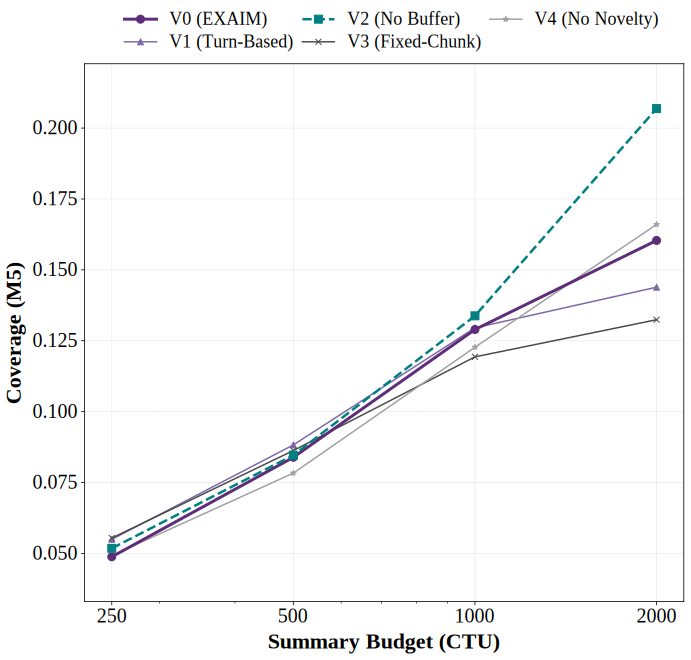
\includegraphics[width=\columnwidth]{saturation/saturation.pdf}
\caption{Budget‑Constrained Coverage (M7). V0 (EXAIM) saturates early; V2 diverges at high budgets.}
\label{tab:budget-coverage}
\end{figure}


To support headline claims with rigorous statistical evidence, we computed paired differences (V0 minus comparator) across the 40 replay cases, bootstrapping to estimate 95\% confidence intervals (Table~\ref{tab:paired-bootstrap}).

\begin{table}[htbp]
\caption{Paired Bootstrap Comparisons (V0 vs. Baselines)}
\begin{center}
\resizebox{\columnwidth}{!}{%
\renewcommand{\arraystretch}{1.3}
\begin{tabular}{lcc}
\toprule
\textbf{Comparison} & \textbf{$\Delta$ Update Count (M1)} & \textbf{$\Delta$ Coverage/Update} \\
\midrule
V0 -- V2 (mean) & --34.75 & +0.0072 \\
CI [low, high] & [--35.1, --34.4] & [+0.0065, +0.0079] \\
\midrule
V0 -- V1 (mean) & +3.15 & --0.0030 \\
CI [low, high] & [+2.9, +3.4] & [--0.0038, --0.0022] \\
\bottomrule
\end{tabular}
}
\label{tab:paired-bootstrap}
\end{center}
\footnotesize
Note: Paired bootstrap: 10k samples, seed=42.
\normalsize
\end{table}

\subsection{Verification Summary}

The experimental results support our core hypotheses regarding event-driven, schema-constrained summarization2. Regarding RQ1a and RQ1b, while raw coverage ($M4$) naturally favors the high-frequency triggering of V2 (0.312 vs. V0's 0.162), a budget-normalized analysis reveals that V0 achieves nearly identical coverage (0.129) to V2 (0.134) at clinician-realistic reading budgets of $\le 1000$ CTU3. Critically, V0 achieves this utility with 75\% fewer interruptions than the high-frequency baseline, representing a reduction of $\Delta M1 = -34.75$ updates per case4. The specific value of semantic gating is further evidenced by V0's novelty filtering, which reduces update frequency by 29\% compared to V4 while incurring only a marginal 8\% coverage cost. Furthermore, V0 achieves 12.5\% higher absolute coverage than the turn-based baseline, V16. For RQ1c and RQ1d, the results demonstrate that syntax-aware buffering produces more groundable content for summarization, as V0 achieved a 26\% improvement in concept-level faithfulness ($M6b = 0.421$) over the 0.333 achieved by V17. The necessity of each architectural primitive is confirmed by the performance of V2, which, despite high raw coverage, creates an unsustainable cognitive burden of 46.4 updates per case. This confirms that the BufferAgent is required to maintain our first design objective's low-interruption requirements9. Collectively, these findings indicate that EXAIM (V0) represents an optimized operating point for clinical deployment, trading middleware computational cost for a substantial reduction in interruption pressure while preserving competitive early-budget information density10



\section{Discussion}

Our findings effectively "close the loop" on the research questions, confirming that DSR-guided middleware can mediate the transparency-efficiency trade-off in streaming AI. We structure the implications of this work into theoretical contributions to design science and practical guidance for clinical deployment.

Under bounded reading budgets, coverage gains from high-frequency updating largely saturate, while interruption burden grows dramatically.

\subsection{Theoretical Implications: Extremes as Design Anchors}

This study extends Design Science Research (DSR) in clinical AI by formalizing the "transparency paradox" as a manageable control problem. 
Historically, CDSS design has oscillated between two extremes: opaque black boxes (high efficiency, low trust) and "firehose" transparency (high trust, cognitive failure). Our ablation results (V0 vs V1/V2) introduce a third stable state: \textbf{Semantic State Transparency}.
By shifting the unit of explanation from the \textit{architectural turn} to the \textit{clinical semantic event}, EXAIM demonstrates that transparency is not a fixed attribute of the model but a tunable variable of the interface. This provides a theoretical design anchor for future multi-agent interfaces: explainability should be decoupled from generation mechanics and governed by an independent logic of clinical meaningfulness.

\subsection{Practical Implications for Workflow Integration}

For practitioners, the success of the BufferAgent logic (V4 vs V0) provides a concrete blueprint for reducing alert fatigue. "Novelty" is often treated as a binary attribute of a fact; however, our results show that in clinical streams, novelty is contextual.
Practically, this implies that CDSS interfaces must stop equating "new token generation" with "new information." The 41\% reduction in updates achieved by novelty filtering suggests that hospitals can deploy multi-agent systems without overwhelming clinicians, provided they implement middleware that actively suppresses redundancy. This shifts the integration burden from the busy clinician (who must currently filter noise) to the automated middleware, directly addressing the workflow compatibility challenge cited in recent reviews \cite{bayor2025cdss}.

\subsection{Deployment Considerations}

To move from artifact to operation, we map EXAIM into the standard four-layer implementation scheme consistent with recent DSR literature:
\begin{enumerate}
    \item \textbf{Data Layer}: Integration with FHIR-enabled EHRs to feed live patient context to upstream agents.
    \item \textbf{Model Layer}: Hosting the multi-agent reasoning engine (e.g., MedAgents) in a secure, HIPAA-compliant enclave.
    \item \textbf{Middleware Layer}: Deploying EXAIM as a low-latency interaction gateway. This layer handles the "contract" capability—ensuring that no matter how erratic the Model Layer behaves, the User Layer receives predictable JSON.
    \item \textbf{User Layer}: A React/Web-based clinician dashboard that subscribes to the EXAIM JSON stream, rendering cards that update in place.
\end{enumerate}
This layered approach isolates the clinical UI from the volatility of LLM generation, ensuring that the tool remains a "decision support" system rather than a "distraction generation" system.

\section{Conclusion}

This paper addressed the challenge of optimizing information density and reducing alert frequency in multi-agent clinical decision support systems. We introduced EXAIM, a novel IT artifact that interposes a middleware layer to transform verbose, interleaved reasoning traces into concise, schema-constrained summaries.
Our solution is built on three validated primitives:
\begin{enumerate}
    \item \textbf{TokenGate}: which enforces syntactic coherence on streaming tokens.
    \item \textbf{BufferAgent}: which filters updates based on semantic novelty and clinical relevance.
    \item \textbf{SummarizerAgent}: which synthesizes content into SBAR/SOAP-aligned structures.
\end{enumerate}

Through systematic DSR evaluation on 40 diagnostic replay cases, we verified that EXAIM represents an effective operating point under clinician-facing constraints. Specifically, paired bootstrap analysis (10,000 samples, seed=42) demonstrates that V0 reduces update burden by 75\% compared to high-frequency baselines (V2) while preserving competitive budget-normalized coverage at reading budgets $\leq$1000 CTU. Compared to turn-based baselines (V1), V0 improves faithfulness by 26\% [0.421 vs 0.333, non-overlapping CIs] and reduces redundancy by 20\% [0.366 vs 0.456]. Importantly, we demonstrated that novelty filtering is essential for preventing update fatigue---V4 (No Novelty) generates 41\% more updates with minimal coverage benefit.

\textbf{Limitations}: Our study is limited by its reliance on retrospective replay data, which, while deterministic, cannot capture real-time clinician behavioral adaptation. Additionally, automated concept-level faithfulness metrics (M6a, M6b) are limited by UMLS NER paraphrase insensitivity and do not perfectly proxy clinical safety or semantic equivalence.

\textbf{Future Work}: Future iterations will focus on three directions: (1) deploying EXAIM in a human-in-the-loop simulation with practicing clinicians to measure decision velocity and usability; (2) expanding the BufferAgent to detect "conflict" events where agents disagree, enabling meta-reasoning transparency; and (3) incorporating entailment-based faithfulness verification to complement concept-overlap metrics.

Ultimately, EXAIM contributes a reproducible architectural pattern for managing the transparency-efficiency trade-off in multi-agent clinical AI, demonstrating that high-velocity reasoning streams can be made observable within human cognitive constraints through principled semantic event detection and schema-constrained synthesis.

\section*{Acknowledgment}

This work was supported by Dakota State University. The authors thank the MAC framework developers for making their diagnostic reasoning traces available for instrumentation.

\bibliographystyle{IEEEtran}
\bibliography{references}

\end{document}




